\section{Anhang}

\subsection{Wie löst man WrStat Übungen?}

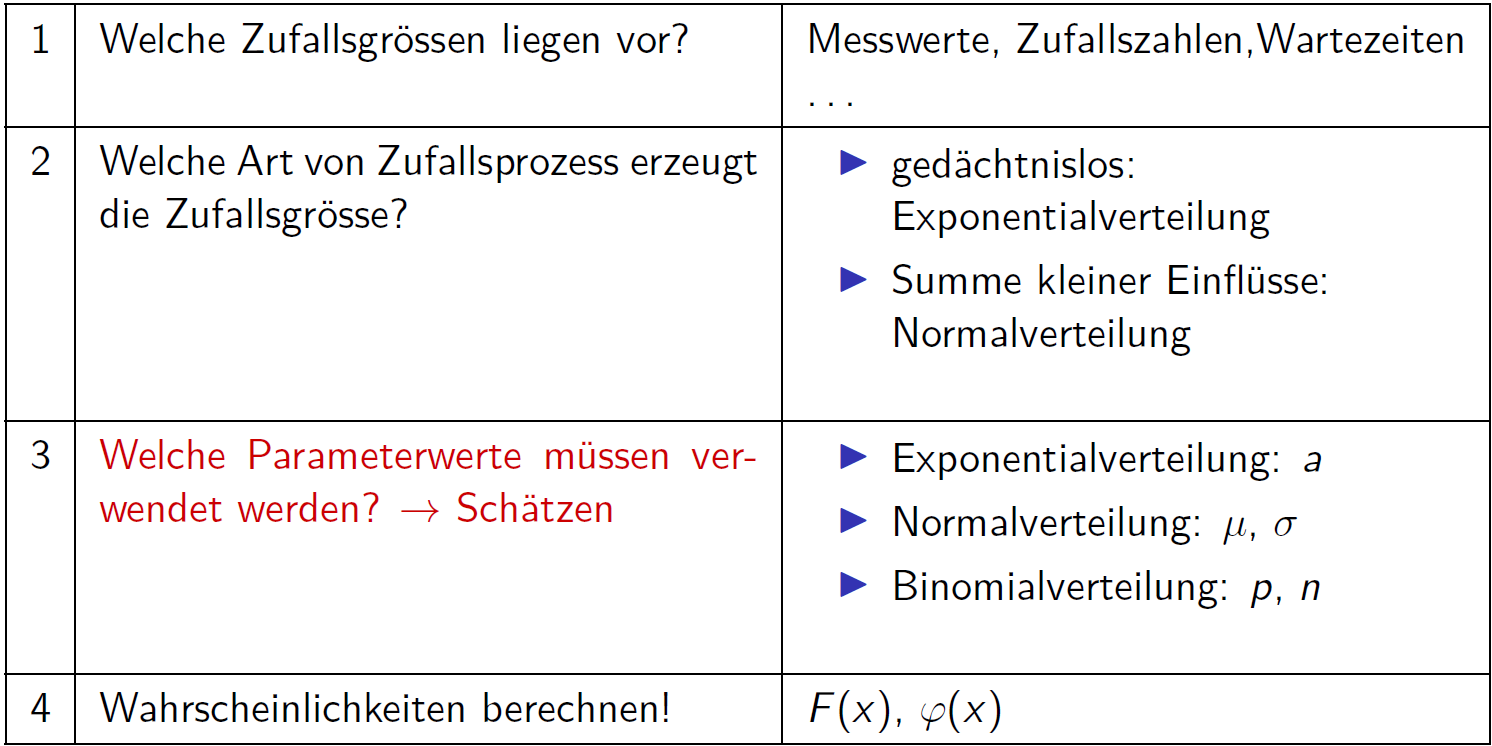
\includegraphics[width=\columnwidth]{images/wrstat_uebungen_loesen.png}

\subsection{Berechnungsformular}

\renewcommand{\arraystretch}{1.5}
\setlength{\tabcolsep}{3pt}
\begin{minipage}[c]{0.56\columnwidth}
\resizebox{\linewidth}{!}{%
\begin{tabular}{|c|c|c|c|c|c|}
	\hline
	$i$ & $x_i$ & $y_i$ & $x_i^2$ & $y_i^2$ & $x_i y_i$ \\ \hline
	$1$ & & & & & \\
	$2$ & & & & & \\
	$\vdots$ & & & & & \\
	$n$ & & & & & \\ \hline
	\color{gray}$\sum$ & \color{gray}$\sum x_i$ & \color{gray}$\sum y_i$ & \color{gray}$\sum x_i^2$ & \color{gray}$\sum y_i^2$ & \color{gray}$\sum x_i y_i$ \\ \hline
	\crd{$\cdot \frac{1}{n}$} & \color{gray}$E(X)$ & \color{gray}$E(Y)$ & \color{gray}$E(X^2)$ & \color{gray}$E(Y^2)$ & \color{gray}$E(XY)$ \\ \hline
\end{tabular}}
\end{minipage}
\hfill
\begin{minipage}[c]{0.42\columnwidth}
\resizebox{\linewidth}{!}{%
\begin{tabular}{|l|l|}
	\hline
	$\var(X)$		& \color{gray}$= E(X^2) - E(X)^2$ \\
	$\var(Y)$		& \color{gray}$= E(Y^2) - E(Y)^2$ \\
	$\cov(X, Y)$	& \color{gray}$= E(XY) - E(X)\,E(Y)$ \\ \hline
	$a$				& \color{gray}$= \cov(X, Y) / \var(X)$ \\
	$b$				& \color{gray}$= E(Y) - a\,E(X)$ \\ \hline
	$r$				& \color{gray}$= \dfrac{\cov(X, Y)}{\sqrt{\var(X) \, \var(Y)}}$ \\[0.8em] \hline
\end{tabular}}
\end{minipage}
\renewcommand{\arraystretch}{1}
\setlength{\tabcolsep}{6pt}

\smallskip
{\small \crd{Attenzione:} $E(\ldots) = \frac{1}{n} \sum_{i=1}^{n} \ldots$ \; (somma della colonna \textbf{diviso} $n$)}

\subsection{Catene di Markov e PageRank}

\subsubsection{Catena di Markov}

Stati $S_j$ (prima della transizione), $S_i^\to$ (dopo la transizione). Matrice di transizione $T$ (omogenea: indipendente dal tempo)
$$ \boxed{ t_{ij} = P(S_i^\to \mid S_j) } \qquad \sum_i t_{ij} = 1 \quad \forall j $$

Distribuzione $p$ con $p_i = P(S_i)$ (probabilità totale):
$$ \boxed{ p' = T \, p } \qquad \boxed{ p(t+n) = T^n \, p(t) } $$


\subsubsection{Distribuzione stazionaria}

\textbf{Perché un eigenvektor?} 

Dopo $n$ passi $p(n) = T^n p_0$. Se per $n \to \infty$ la distribuzione converge a $p$, un passo in più non cambia nulla: la probabilità ``dopo'' è uguale a quella ``prima'', $P(S_i^\to) = P(S_i)$, cioè $p' = p$. \\
Con $p' = T\,p$ segue $T\,p = 1 \cdot p$ \textrightarrow\ \textbf{eigenvektor con eingwert $1$}


\begin{tabular}{ll}
	stazionaria			& $T \, p = p$ \textrightarrow\ eigenvektor con eingwert $1$ \\
	distribuzione limite	& $\displaystyle \lim_{n \to \infty} T^n p_0 = p$ (è stazionaria)
\end{tabular}



\subsubsection{Google PageRank}

$S_j$ = visitatori sulla pagina $j$, $S_i^\to$ = visitatori sulla pagina $i$ dopo la navigazione

\textbf{Matrice dei link} $H$ \quad ($h_{ij} = P(S_i^\to \mid S_j)$ = probabilità di andare dalla pagina $j$ alla pagina $i$, somma delle colonne $1$):
$$ \boxed{ H = \begin{pmatrix}
	P(S_1^\to \mid S_1) & \cdots & P(S_1^\to \mid S_N) \\
	\vdots & \ddots & \vdots \\
	P(S_N^\to \mid S_1) & \cdots & P(S_N^\to \mid S_N)
\end{pmatrix} } $$

Libero arbitrio $F$ (l'utente non segue un link), peso $\omega$ per la navigazione tramite link:
$$ \boxed{ G = \omega \, H + (1-\omega) \, \frac{1}{N} A } \qquad A = \begin{pmatrix} 1 & \cdots & 1 \\ \vdots & & \vdots \\ 1 & \cdots & 1 \end{pmatrix} $$

\textbf{PageRank} = autovettore $p$ di $G$ con autovalore $1$:
$$ \boxed{ G \, p = p } \qquad p = \lim_{n \to \infty} G^n p_0 $$